%! TEX root=../main.tex
\section{Commutative Algebra}

\subsection{ED, PID and UFD (week 9)}

We shall consider $R$ to be an integral domain below.
\begin{definition}
  A function $N: R \to \Nb$ with $N(0) = 0$ is called a norm on $R$.
\end{definition}

\begin{definition}
  $R$ is called a Euclidean domain if exists a norm $N$ on $R$
  satisfying
  \[ \forall a, b \in R, \ \exists q, r \in R \text{ s.t. }
  a = qb + r \text{ with } r = 0 \text{ or } N(r) < N(b) \]
\end{definition}

\begin{example} \hfill
  \begin{itemize}
    \item $\Zb$ is a ED with $N(n) = \abs{n}$.
    \item $K[x]$ is a ED with $N(f) = \deg f, \, \forall f \in K[x]$.
  \end{itemize}
\end{example}

\begin{definition}
  $A_d$ is defined to be the ring of integers in the quadratic field $\Qb(\sqrt{d})$
  with $d \neq 1$ and $d$ is square-free. That is,
  \[ A_d \triangleq \Set{ \alpha \in \Qb(\sqrt{d}) \mid \alpha \text{ is integral over } \Zb} \]
\end{definition}

\begin{theorem} \hfill
  \begin{itemize}
    \item If $d \equiv 1 \pmod{4}$, then
      \[ A_d = \Set*{ a + b \frac{1 + \sqrt{d}}{2} : a, b \in \Zb } \]
    \item Else, $d \equiv 2, 3 \pmod{4}$, then
      \[ A_d = \Set{ a + b \sqrt{d} : a, b \in \Zb } \]
  \end{itemize}
  \begin{proof}
    Let $\alpha = p + q \sqrt{d} \in A_d$ for $p, q \in \Qb$ with $q \neq 0$.
    We have $\alpha - p = q \sqrt{d}$, then $(\alpha - p)^2 = q^2 d$
    and thus $\alpha^2 - 2p\alpha + (p^2 - q^2d) = 0$.
    Let $g(x) \triangleq x^2 - 2px + (p^2 - q^2 d)$.
    Assume $f(x) \in \Zb[x]$ with $f$ monic and $f(\alpha) = 0$, then
    we could write $f(x) = q(x) g(x) + (ax + b)$.
    Since $\alpha$ is not rational, $a\alpha+b = 0 \implies a = b = 0$,
    so $f(x) = q(x) g(x)$ in $\Qb[x]$. By gauss lemma,
    $g(x) \in \Zb[x]$, so $2p \in \Zb$ and $p^2 - q^2 d \in \Zb$.

    If $2p$ is even, then $p \in \Zb$, and $p^2 - q^2 d \in \Zb$
    implies $q$ is also an integer since $d$ is square free.

    If $2p$ is odd, say $2p = 2m+1$, then $(2p)^2 \equiv (2m+1)^2 \equiv 1 \pmod{4}$.
    Also, $4(p^2 - q^2 d) \equiv 0 \pmod{4}$, so $4q^2d \equiv 4p^2 \equiv 1 \pmod{4}$.
    Since $d$ is square free, so $4 \nmid d$, thus $q$ has to be of the form
    $q = (2n+1)/2$. Plug in the equation we get $d \equiv 1 \pmod{4}$.
    Thus in this case, $p, q$ are half integer and $d \equiv 1 \pmod{4}$.
  \end{proof}
\end{theorem}

\begin{theorem}
  $A_d$ is a ED if $d = 2, 3, 5, -1, -2, -3, -7, -11$. Hence $A_d$ is also PID and UFD
  for these value.
  \begin{proof}
    Let $N'(p + q\sqrt{d}) = (p + q\sqrt{d})(p - q\sqrt{d}) = p^2 - q^2 d$.
    Define $N(\alpha) \triangleq \abs{N'(\alpha)}$ which is positive
    since $p^2 - q^2 d = 0 \iff p = q = 0$. Notice also $N$
    is multiplicative.

    Now, for $\alpha, \beta \in A_d$, write $\alpha/\beta = x+y\sqrt{d}$.
    If we could find $\lambda = a+b\sqrt{d}$ such that
    $\abs{\alpha / \beta - \lambda} < 1$, then
    $\alpha = \beta \lambda + \gamma$ with $N(\gamma) < N(\beta)$
    which proves that $A_d$ is an ED.

    \begin{itemize}
      \item $d = 2, 3, -2, -1$:
        Choose $a, b \in \Zb$ such that
        $\abs{x - a}, \abs{y - b} \leq 1/2$.
        Then $N \triangleq N(\alpha/\beta - \lambda) = \abs{(x - a)^2 - (y-b)^2d}$.
        \begin{itemize}
          \item If $d = 2, 3$, then $N \leq \max(\abs{(x - a)^2}, \abs{(y-b)^2d}) \leq
            \max(1/4, d/4) < 1$.
          \item If $d = -2, -1$, then $N \leq \abs{(x - a)^2} + \abs{(y-b)^2d} \leq
            1/4 + \abs{d}/4 < 1$.
        \end{itemize}
      \item $d = 5, -3, -7, -11$: Similarly, but now $d \equiv 1 \pmod{4}$,
        so we could choose $\lambda = a + b(1 + \sqrt{d})/2 = (a + b/2) + b/2 \sqrt{d}$.
        Thus let $b$ be the one such that $\abs{2y - b} \leq 1/2$, and
        then choose $a$ so that $x - a - b/2 \leq 1/2$.
        We have $N(\alpha/\beta - \lambda) = \abs{(x - a - b/2)^2 - d (y - b/2)^2}
        \leq 1/4 + d/16 < 1$.
    \end{itemize}
  \end{proof}
\end{theorem}

\begin{example}
  $A_{-5}$ is not a ED.

  \begin{proof}
    Consider $6 = 2 \cdot 3 = (1 + \sqrt{-5})(1 - \sqrt{-5})$.
    Notice that $1 + \sqrt{-5}$ is irreducible, since if $1 + \sqrt{-5} = \alpha \beta$,
    then $6 = N(1 + \sqrt{-5}) = N(\alpha) N(\beta)$. But this implies
    $a^2 + 5b^2 = 2 \text{ or } 3$ which has no integer solution.
    Also $1 + \sqrt{-5} \nmid 2, 3$. Since if $(1 + \sqrt{-5}) \alpha = 2$,
    then $N(1 + \sqrt{-5}) N(\alpha) = N(2) = 4$, but $N(1 + \sqrt{-5}) = 6$.
    Similarly $1 + \sqrt{-5} \nmid 3$. So $A_{-5}$ is not an UFD thus not an ED.
  \end{proof}
\end{example}

\subsubsection{$A_{-1}$ and $A_{-3}$}

\begin{definition}
  If $p$ is odd and $a \not\equiv 0 \pmod{p}$, then
  \begin{itemize}
    \item If $x^2 \equiv a \pmod{p}$ is solvable, then define $\left( \frac{a}{p} \right) = 1$.
    \item Else $x^2 \equiv a \pmod{p}$ is not solvable and define $\left( \frac{a}{p} \right) = -1$.
  \end{itemize}
\end{definition}

\begin{prop} \hfill
  \begin{itemize}
    \item $a \equiv b \pmod{p} \implies \left( \frac{a}{p} \right) = \left( \frac{b}{p} \right)$.
    \item $\left( \frac{a}{p} \right) = a^{(p-1)/2}$:
      \begin{proof}
      Consider the sequence:
      \[ \begin{tikzcd}[row sep = 0]
          1 \ar[r] & (\Fb_p^\times)^2 \ar[r] & \Fb_p^\times \ar[r, "\varphi"] & \Set{\pm 1} \ar[r] & 1 \\
          & y^2 \ar[r, mapsto] & y^2=x \ar[r, mapsto] & (-1)^{(p-1)/2} \ar[r, mapsto] & 1 \\
      \end{tikzcd} \]
      which is exact since $y^2 \mapsto y^2 \mapsto y^{2 (p-1)/2} \equiv 1$.
      And since $\Fb_p^\times$ is cyclic with even elements,
      $\big[\Fb_p^\times: (\Fb_p^\times)^2 \big] = 2$, and $(\Fb_p^\times)^2 = \ker \varphi$.
      \end{proof}
    \item $\left( \frac{ab}{p} \right) = \left( \frac{a}{p} \right) \left( \frac{b}{p} \right)$.
    \item Let $t_k \equiv ka \pmod{p}$ with $0 \leq t_k < p$, for $1 \leq k \leq (p-1)/2$.
      Assume that $n = \# \Set{t_i \mid t_i > p/2}$, then $\left(\frac{a}{p}\right) = (-1)^n$.
      \begin{proof}
        Define
        \[ \abs{t_i} = \begin{cases}
            t_j & \text{ If } 1 \leq t_j < p/2 \quad (t_j \equiv \abs{t_j}) \\
            p - t_j & \text{ If } p/2 < t_j < p \quad (t_j \equiv -\abs{t_j})
        \end{cases} \]
      Notice that $\abs{t_i}$ takes value between $1$ and $(p-1)/2$,
      and $\abs{ra} \equiv \abs{sa} \pmod{p} \implies
      ra \equiv \pm sa \pmod{p} \implies r \equiv \pm s \pmod{p}$ since $\gcd(a, p) = 1$.
      So $\abs{t_k}$ would have distinct value for $1 \leq k \leq (p-1)/2$.
      Thus
      \[ \prod t_k \equiv \frac{p-1}{2}! a^{(p-1)/2} \equiv (-1)^n \frac{p-1}{2}!
        \implies a^{(p-1)/2} \equiv (-1)^n \]
      \end{proof}
    \item If $p, q$ are odd primes, then we have:
      \[ \left( \frac{q}{p} \right) = (-1)^{\left( \sum_{k=1}^{(p-1)/2} \floor*{\frac{kq}{p}} \right)} \]
      \begin{proof}
        Write $kq = g_k p + t_k$ with $0 \leq t_k < p$ consistent with the previous definition.
        Then we have $\floor{kq / p} = g_k$, and
        \begin{alignat*}{4}
          & \text{ if } \abs{t_k} = t_k && \leadsto qk = g_k p + \abs{t_k} &&
          \leadsto k \equiv g_k + \abs{t_k} \pmod{2} \\
          & \text{ if } \abs{t_k} = p - t_k \quad && \leadsto qk = (g_k+1) p - \abs{t_k} \quad &&
          \leadsto k \equiv g_k + 1 + \abs{t_k} \pmod{2} \\
        \end{alignat*}
        So
        \[ \sum_{i = 1}^{(p-1)/2} k \equiv n + \sum_{i=1}^{(p-1)/2} \floor*{\frac{qk}{p}}
          + \sum_{k=1}^{(p-1)/2} \abs{t_k} \pmod{2} \]
        As in the previous proof, $\sum k = \sum \abs{t_k}$, so $n \equiv \sum \floor{qk/p} \pmod{2}$,
        which proves the statement.
      \end{proof}
    \item
      \[ \left( \frac{p}{q} \right) \left( \frac{q}{p} \right)
        = (-1)^{\left(\frac{p-1}{2}\right) \left(\frac{q-1}{2}\right)} \]
      By above,
      \[ \left( \frac{p}{q} \right) \left( \frac{q}{p} \right)
        = (-1)^{\left( \sum_{k=1}^{(p-1)/2} \floor*{\frac{kq}{p}} \right)}
        (-1)^{\left( \sum_{k=1}^{(q-1)/2} \floor*{\frac{kp}{q}} \right)} 
      \]
      Which is the number of integer points in the rectangle:
      \begin{figure}[H]
        \centering
        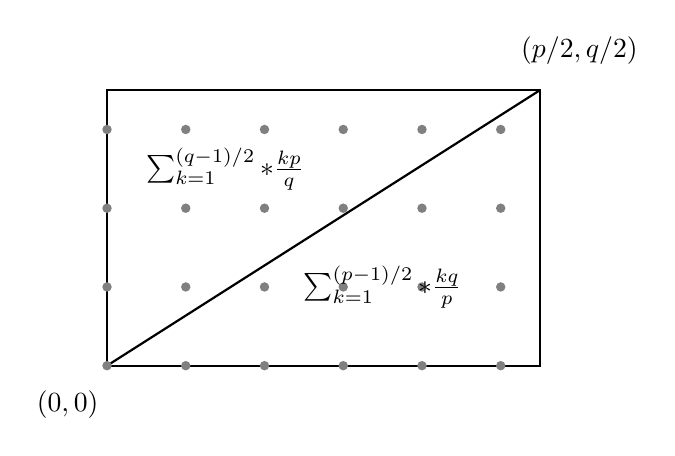
\begin{tikzpicture}
          \draw[thick] (0, 0) rectangle (5.5, 3.5);
          \draw[thick] (0, 0) -- (5.5, 3.5);
          \foreach \x in {0, ..., 5} {
            \foreach \y in {0, ..., 3}
            \fill[black!50] (\x, \y) circle (0.06);
          }
          \node at (1.5, 2.5) {$\sum_{k=1}^{(q-1)/2} \floor*{\frac{kp}{q}}$};
          \node at (3.5, 1) {$\sum_{k=1}^{(p-1)/2} \floor*{\frac{kq}{p}}$};
          \node at (-.5, -.5) {$(0, 0)$};
          \node at (6, 4) {$(p/2, q/2)$};
        \end{tikzpicture}
      \end{figure}
      And we know that there are $\frac{p-1}{2} \frac{q-1}{2}$ points in the rectangle.
  \end{itemize}
  % TODO missing something...
\end{prop}
% TODO missing something...

\begin{prop}
  \begin{itemize}
    \item $\alpha$ is a unit $\iff$ $N(\alpha) = 1$.
      \begin{proof}
        ``$\Rightarrow$": If $\alpha \beta = 1$, $N(\alpha) N(\beta) = 1$ so $N(\alpha) = 1$.

        ``$\Leftarrow$": Immediately by $\alpha \bar{\alpha} = N(\alpha) = 1$.
      \end{proof}
    \item If $\alpha$ is a prime in $A_d$, then $N(\alpha) = p \text{ or } p^2$
      for some prime integer $p$. Also $N(\alpha) = p^2 \implies \alpha \sim p$.
      \begin{proof}
        $\alpha \bar{\alpha} = N(\alpha) = p_1 \dotsm p_n$ where $p_i$ are
        primes in $\Zb$. Continue using the fact that ``If $\alpha$
        is a prime and $\alpha \mid xy$, then $\alpha \mid x$ or $\alpha \mid y$'',
        we will get $\alpha \mid p_i$ for an $i$. Say $\alpha \beta = p_i$,
        then $\bar{\alpha}\bar{\beta} = \bar{p}_i = p_i$,
        so $N(\alpha) N(\beta) = p_i^2$ which means that $N(\alpha) = p_i \text{ or } p_i^2$.
        Also, if $N(\alpha) = p_i^2$, then $N(\beta) = 1 \implies \beta \text{ is a unit }$.
      \end{proof}
  \end{itemize}
\end{prop}

By the proposition above we identify the unit in $A_{-1}, A_{-3}$.
\begin{itemize}
  \item $A_{-1}$: $\pm 1, \pm \mathrm{i}$.
  \item $A_{-3}$: $\pm 1, \pm \omega, \pm \omega^2$.
\end{itemize}

Now, notice that $2 = (1 + \sqrt{-1})(1 - \sqrt{-1})$, $3 = (1 - \omega) (1 - \omega^2)$,
so $2, 3$ are not prime in $A_{-1}, A_{-3}$ respectively.

Let $p$ be a prime in $\Zb$.
\begin{itemize}
  \item In $A_{-1}$:
    \begin{align*}
      & p \text{ is a prime in } \Zb[\sqrt{-1}] \\
      \iff \ & \gen{p} \text{ is maximal ideal } \\
      \iff \ & \frac{\Zb[\sqrt{-1}]}{\gen{p}} \cong \frac{\Zb[x]}{\gen{p, x^2+1}}
      \cong \frac{\Zb[x]/\gen{p}}{\gen{p, x^2+1}/\gen{p}} \cong \frac{\Fb_p[x]}{x^2+1}
      \text{ is a field } \\
      \iff \ & x^2 + 1 \text{ irreducible in } \Fb_p[x] \\
      \iff \ & x^2 \equiv -1 \pmod{p} \text{ is not solvable } \\
      \iff \ & \left(\frac{-1}{p}\right) = (-1)^{(p-1)/2} \neq 1 \\
      \iff \ & p \not\equiv 1 \pmod{4}
    \end{align*}
    So $p$ is {\bf not} a prime in $A_{-1}$ $\iff$ $p \equiv 1 \pmod{4}$.
  \item In $A_{-3}$: 
    If a prime $p \neq 3$ in $\Zb$ is not a prime in $\Zb[\omega]$, then it has
    a nontrivial factor $\alpha \mid p$. But $N(p) = p^2$, so 
    we must have $N(\alpha) = p$, i.e. $\alpha \bar{\alpha} = p$.
    Let $\alpha = a + b \omega$, then
    $p = \alpha \bar{\alpha} = a^2 + b^2 - ab \implies 4p = (2a - b)^2 + 3b^2$,
    so $p \equiv (2a - b)^2 \equiv 1 \pmod{3}$. ($p \not\equiv 0$ since $p \neq 3$)

    Conversely, if $p \equiv 1 \pmod{3}$, then
    \[ \left(\frac{-3}{p}\right)
      = \left(\frac{-1}{p}\right) \left(\frac{3}{p}\right)
      = (-1)^{(p-1)/2} \left(\frac{p}{3}\right) (-1)^{\frac{p-1}{2} \cdot \frac{3-1}{2}}
      = \left(\frac{p}{3}\right) = \left(\frac{1}{3}\right) = 1 \]
    So exists $a \in \Zb$ such that $a^2 \equiv -3 \pmod{p}$,
    say $pb = a^2 + 3 = (a + \sqrt{-3}) (a - \sqrt{-3}) = (a+1 + 2\omega) (a - 1 - 2\omega)$.

    If $p$ is a prime in $\Zb[\omega]$, then $p \mid (a+1+2\omega)$ or $p \mod (a - 1 - 2\omega)$,
    which implies that $p \mid 2$ (since $p \in \Zb$, $p \mid a + b\omega \implies p \mid a, p \mid b$), 
    which leads to a contradiction, thus $p$ is not a prime.

    Hence $p \neq 3$ is not a prime in $A_{-3}$ $\iff$ $p \equiv 1 \pmod{3}$.
\end{itemize}


\subsection{Primary decomposition}
\begin{definition} \hfill
  \begin{itemize}
    \item The radical of an ideal $I$ is defined by $\sqrt{I} =
      \Set{ a \in R \mid a^n \in I \text{ for some } n \in \Nb}$.
    \item $I$ is radical if $\sqrt{I} = I$.
  \end{itemize}
\end{definition}

\begin{definition}
  The {\bf nilradical}\index{nilradical} is defined as $\sqrt{\gen{0}} \triangleq
  \Set{ a \in R \mid a^n = 0 \text{ for some } n \in \Nb}$.
  Elements in it are called nilpotent.
\end{definition}

\begin{prop}
  $\sqrt{ \gen{0} } = \bigcap\limits_{P \in \Spec R} P$, where $\Spec R$ is the
  set of prime ideals in $R$.

  \begin{proof}
    ``$\subset$'': Notice that $a^n = 0 \in P$ for any prime ideal $P$. By the definition of
    prime ideal, either $a \in P$ or $a^{n-1} \in P$. No matter which, eventually we would get
    $a \in P$.

    ``$\supset$'':
    Let $\Sc \triangleq \Set{ I : \text{ ideal in } R \given a^n \notin I, \, \forall n \in \Nb}$.
    By the routine argument of Zorn's lemma, exists maximal element $Q$ in $\Sc$.
    We claim that $Q$ is a prime ideal.

    For each $x, y \notin Q$, we have $Q + Rx \supsetneq Q$ and $Q + Ry \supsetneq Q$.
    By the maximality of $Q$, these two ideals are not in $\Sc$.
    So exists $n, m$ such that $a^n \in Q + Rx,\, a^m \in Q + Ry$ which implies
    $a^{n+m} \in Q + Rxy$, so $Q + Rxy \notin \Sc$, thus $xy \notin Q$,
    hence $Q$ is prime.
  \end{proof}
\end{prop}

\begin{coro} \label{coro:equation-of-sqrt-ideal}
  \[ \sqrt{I} = \bigcap_{\substack{P \supset I \\ P \in \Spec R}} P \]

  \begin{proof}
    Notice that $\Spec \quot{R}{I} = \Set{P \in \Spec R \mid R \subset I}$.
    By the proposition above,
    \[
      \sqrt{\langle \bar0 \rangle} = \bigcap_{\bar{P} \in \Spec \quot{R}{I}} \bar{P}
      \quad \implies \quad \sqrt{I} = \bigcap_{\substack{P \supset I \\ P \in \Spec R}} P
      \qedhere
    \]
    \end{proof}
\end{coro}

\begin{definition}
  An ideal $q$ of $R$ is called primary if $q \neq R$ and ``$xy \in q$ and $x \notin q$''
  implies $y^n \in q$ for some $n \in \Nb$.
\end{definition}

\begin{prop} \hfill
  \begin{itemize}
    \item $\text{prime} \implies \text{primary}$.
    \item $\sqrt\text{primary} \implies \text{prime}$. Also, if $q$ is primary, then $p = \sqrt{q}$
      is the smallest prime ideal containing $q$, we say $q$ is $p$-primary.
  \end{itemize}

  \begin{proof}
    The first one is obvious.

    If $q$ is primary and $\sqrt{q} = p$. For any $xy \in p$ and $x \notin p$,
    there exists $n$ so that $x^n y^n \in q$, and for this $n$, $x^n \notin q$.
    Thus $(y^n)^m \in q$ for some $m$, hence $y \in p$. We conclude that $p$ is a prime ideal.

    Finally, by corollary~\ref{coro:equation-of-sqrt-ideal},
    \[ p = \sqrt{q} = \bigcap_{\substack{P \supset q \\ P \in \Spec R}} P \subset P,
    \quad \forall P \text{ prime }, \]
    thus $p$ is indeed the smallest.
  \end{proof}
\end{prop}

\begin{example}
  The primary ideals in $\Zb$ are $\langle 0 \rangle$ and $\langle p^m \rangle$
  where $p$ is a prime.

  \begin{proof}
    If $q = \langle a \rangle$ is primary, then $\sqrt{q} = \langle p \rangle$ is
    prime, and $p^n \in \langle a \rangle$. So $ab = p^n$ which implies $a = p^m$
    for some $m$.
  \end{proof}
\end{example}

\begin{definition}
  An ideal $I$ is said to be {\bf irreducible} \index{Ideal!irreducible}
  if $I = q_1 \cap q_2 \implies I = q_1 \lor I = q_2$.
\end{definition}

\begin{definition}
  Define $(I: x) = \Set{ a \in R \mid ax \in I}$.
\end{definition}

\begin{theorem} \label{thm:noeth-irr-ideal-is-primary}
  In a Noetherian ring $R$, every irreducible ideal $I$ is primary.

  \begin{proof}
    Let $xy \in I$ and $x \notin I$. Consider $(I : y) \subseteq (I: y^2) \subseteq \dotsm$.
    Since $R$ is Noetherian, exists $n$ such that $(I: y^n) = (I: y^m)$ for any $m \geq n$.

    We claim that $I = (I + Ry^n) \cap (I + Rx)$.
    \begin{itemize}
      \item ``$\subset$'': Obvious.
      \item ``$\supset$'': For any $b \in (I + Ry^n) \cap (I + Rx)$,
        write $b = a_1 + r_1 y^{n} = a_2 + r_2 x$. Then
        $r_1 y^{n+1} = a_2 y - a_1 y + r_2 x y \in I$ since $a_1, a_2, xy \in I$.
        So $r_1 \in (I: y^{n+1}) = (I: y^n) \implies r_1 y^n \in I$.
        Thus $b = a_1 + r_1 y^n \in I$.
    \end{itemize}

    Now by the fact that $I$ is irreducible and $I \neq I + Rx$ since $x \notin I$,
    thus $I = I + Ry^n \implies y^n \in I$.
  \end{proof}
\end{theorem}

\begin{theorem} \label{thm:noeth-ideal-is-finite-intersection}
  In a Noetherian ring $R$, every ideal is a finite intersection of irreducible ideals.

  \begin{proof}
    If not, let $\Ic \triangleq \Set{I: \text{ ideal in } R \mid I \text{ is not a finite intersection
        of irreducible ideals }}$ and $\Ic$ is not an empty set.
    Since $R$ is Noetherian, the set has a maximal element $I_0$. Then $I_0$ is not
    irreducible (or else it is an intersection of itself, which is irreducible).
    Write $I_0 = I_1 \cap I_2$, with $I_1, I_2 \neq I_0$. Then $I_1, I_2 \notin \Ic$,
    so these two ideals could be written as a finite intersection of irreducible ideals,
    implying that $I_0$ could also be written as a finite intersection of irreducible ideals,
    which is a contradiction.
  \end{proof}
\end{theorem}

\begin{prop} \label{prop:primary-divide-by-element}
  Let $q$ be a $p$-primary ideal and $x \in R$.
  \begin{enumerate}
    \item If $x \in q$, then $(q: x) = R$.
      \begin{proof}
        In this case $1 \in (q: x)$, thus $(q: x) = R$.
      \end{proof}
    \item If $x \notin q$, then $(q: x)$ is $p$-primary.
      \begin{proof}
        For any $y \in (q: x)$, $xy \in q$ but $x \notin q$, thus $y^n \in q \implies y \in p$.
        Hence
        \[ q \subset (q: x) \subset p \implies p = \sqrt{q} \subset \sqrt{(q: x)} \subset \sqrt{p} = p \]
        and thus $(q: x)$ is $p$-primary.

        For any $y, z$ with $yz \in (q: x)$ but $y \notin (q: x)$, which is equivalent
        to $xyz \in q$ but $xy \notin q$. Since $q$ primary, $z^n \in q \subset (q: x)$.
      \end{proof}
    \item If $x \notin p$, then $(q: x) = q$.
      \begin{proof}
        \[
          \left\{ \begin{array}{l}
            y \in (q: x) \\
            x \notin p \\
          \end{array} \right. \implies
          \left\{ \begin{array}{l}
            xy \in (q: x) \\
            x^n \notin q, \ \forall n \in \Nb \\
          \end{array} \right. \implies y \in q
          \qedhere
        \]
      \end{proof}
  \end{enumerate}
\end{prop}

\begin{prop}  \label{prop:intersection-of-primary-is-primary}
  If each $q_i$ are $p$-primary, then $q \triangleq \cap_{i = 1}^n q_i$ is $p$-primary.

  \begin{proof}
    We check that $\sqrt{q} = \bigcap_{i = 1}^n \sqrt{q_i} = \bigcap_{i = 1}^n p = p$.

    Also, if $xy \in q$ with $x \notin q$, then $x \notin q_k$ for some $k$.
    But $xy \in q_k$, thus $y^n \in q_k$.
    But $q_k \subseteq \sqrt{q_k} = p = \sqrt{q}$, so $(y^n)^{m'} = y^m \in q$, 
    thus $q$ is $p$-primary.
  \end{proof}
\end{prop}

\begin{definition}
  A {\bf primary decomposition} of $I = q_1 \cap \dots \cap q_n$ is {\bf minimal} if $\sqrt{q_1}, \dots, \sqrt{q_n}$
  are distinct and $q_i \not\supseteq \bigcap_{j \neq i} q_j$.
\end{definition}

A minimal primary decomposition of an ideal always exists in Noetherian ring since by
theorem~\ref{thm:noeth-ideal-is-finite-intersection}, the ideal could be written
as a finite intersection of irreducible ideals, and then by theorem~\ref{thm:noeth-irr-ideal-is-primary},
these ideals are primary. Now If $\sqrt{q_i} = \sqrt{q_j}$ happen in these ideals,
we could remove these two ideals and add $q' = \sqrt{q_i} \cap \sqrt{q_j}$.
By proposition~\ref{prop:intersection-of-primary-is-primary}, $q'$ is also primary.
And if $q_i \supseteq \bigcap_{j \neq i} q_j$, we could simply remove $q_i$.

\medskip

\begin{theorem}[Uniqueness of primary decomposition]
  Let $I = \cap_{i = 1}^n q_i$ be a minimal decomposition of $I$.
  If $p_i = \sqrt{q_i}, \, \forall i$, then we have
  \[ \Set{p_i} = \Set[\Big ]{ \sqrt{(I: x)} \given x \in R \land \sqrt{(I: x)} \in \Spec R } \]
  which is independent of the decomposition.

  \begin{proof}
    ``$\supset$'': Let $x \in R \setminus I$, then $(I: x) = \big( \bigcap_{i=1}^n q_i : x \big)
    = \bigcap_{i = 1}^n (q_i: x)$. By proposition~\ref{prop:primary-divide-by-element},
    we have $\sqrt{(I: x)} = \bigcap \sqrt{(q_i: x)} = \bigcap_{x \notin q_i} p_i$.

    Now, we have the following observation. ``If $p \in \Spec R$ with $p = \bigcap_{i=1}^n J_i$,
    then $p = J_j$ for some $j$.'' If not, then $J_i \not\subset p$ for all $i$,
    so we could pick $x_i \in J_i \setminus p$.
    But then $x_1 x_2 \dotsm x_n \in \cap J_i \in p$ since $J_i$ are ideals,
    which leads to a contradiction since $p$ is prime.

    So if $\sqrt{(I: x)}$ is a prime, then it is equal to some $p_i$.

    ``$\subset$'': By assumption, $q_i \not\supseteq \bigcap_{j \neq i} q_j$ for each $i$,
    thus we could pick $x \in \bigcap_{j \neq i} q_j \setminus q_i$,
    then $\sqrt{(I: x)} = \bigcap_j \sqrt{(q_j: x)} = \sqrt{(q_i: x)} = p_i$.
  \end{proof}
\end{theorem}

\begin{definition}
  If $\Set{p_i}$ is the unique prime ideals from the minimal primary decomposition of $I$.
  \begin{itemize}
    \item $\Set{p_i}$ is said to be associated with $I$ or to belong to $I$.
    \item The minimal elements in $\Set{p_i}$ are called isolated primes.
    \item The other are called embedded primes.
  \end{itemize}
\end{definition}

\begin{example}
  Let $R = k[x, y]$ and $I = \gen{ x^2, xy }$. If $P_1 = \gen{x},
  P_2 = \gen{ x, y }$, then $I = P_1 \cap P_2^2$.
  $P_1$ is isolated, while $P_2$ is embedded.
\end{example}
